\documentclass[../../../main.tex]{subfiles}

\begin{document}

This section was mostly inspired by \cite{Sun2023}.

\subsubsection{Uniform Hopping: Towards the Square Lattice}

I investigate the effect of uniformly varying hopping amplitudes with one edge case reproducing a lattice topolgically equivalent to the square lattice. . I modify the hopping amplitudes in the unit cell of the two-site unit cell as follows 

\begin{center}
	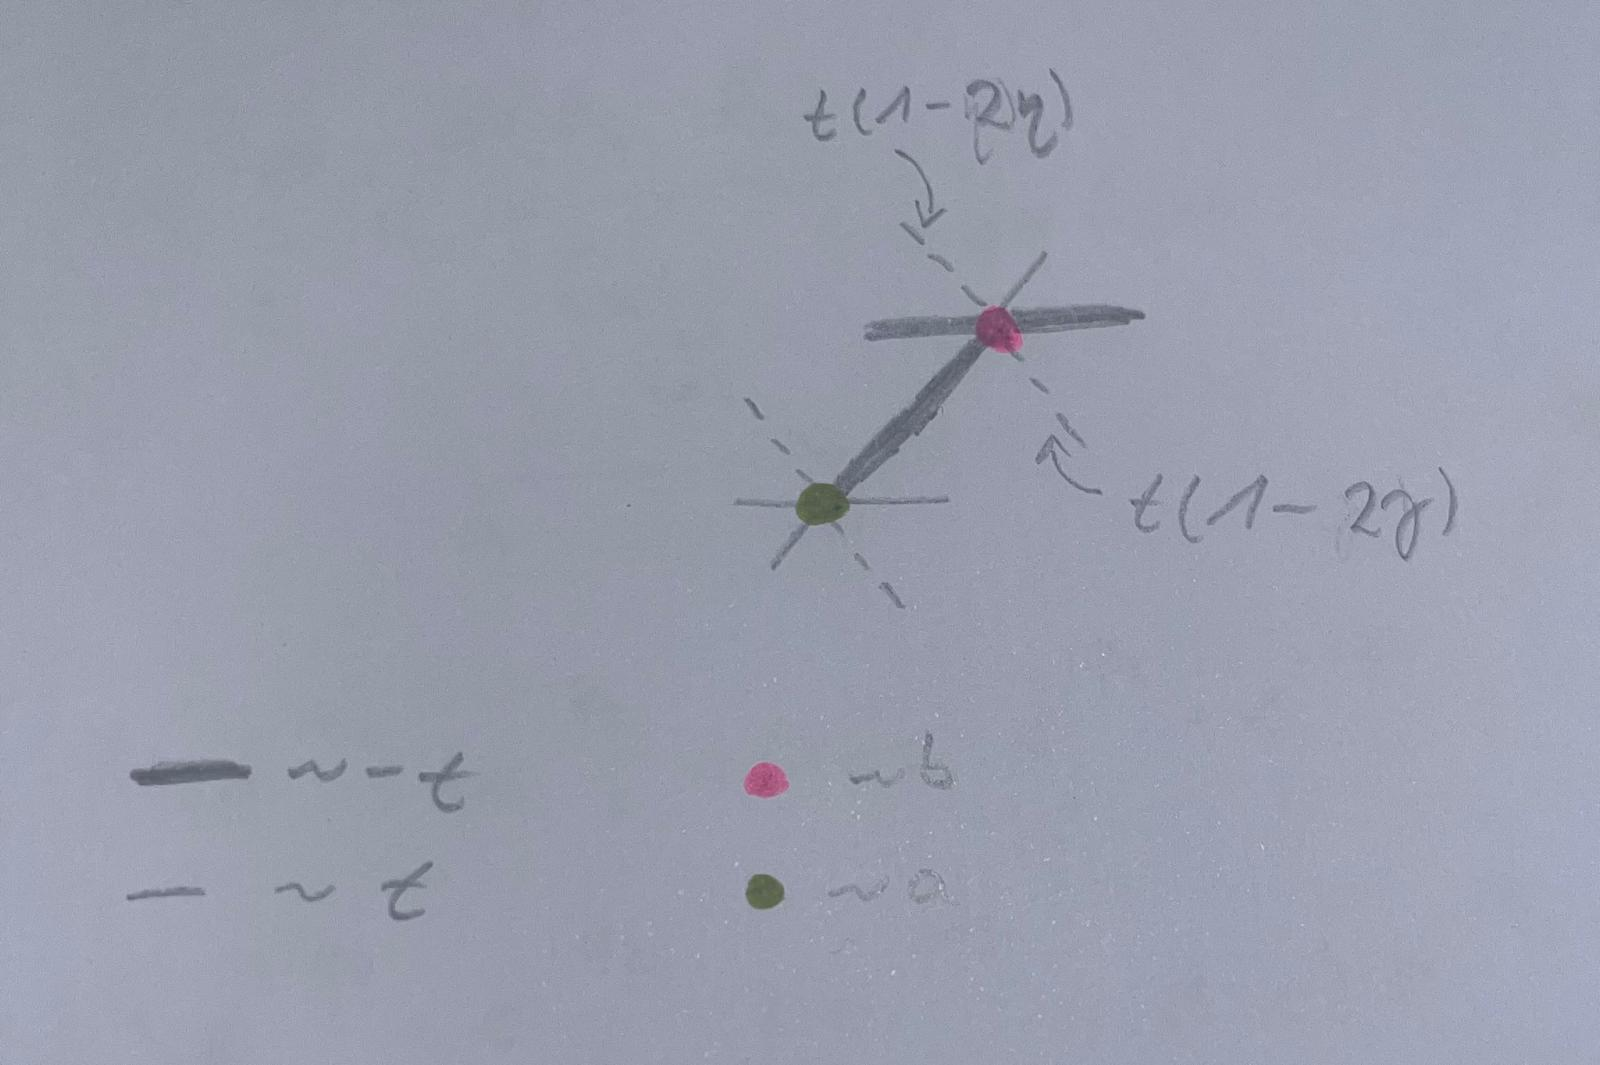
\includegraphics[width = \textwidth]{uniform_hopping_games.jpeg}
\end{center}

This gives the real space Hamiltonian 

\begin{align}
	\begin{split}
		H = t \sum_{i\sigma}\bigg(&-b_{i\sigma}^\dagger b_{i+t_1;\sigma} - b_{i\sigma}^\dagger b_{i-t_1;\sigma} + a_{i\sigma}^\dagger a_{i+t_1;\sigma} + a_{i\sigma}^\dagger a_{i-t_1;\sigma} \\
		&- b_{i\sigma}^\dagger a_{i\sigma} + b_{i\sigma}^\dagger a_{i+t_2;\sigma} + (1-2\eta)b_{i\sigma}^\dagger a_{i-t_1+t_2;\sigma} + (1-2\gamma) b_{i\sigma}^\dagger a_{i+t_1}  \\
		&-a_{i\sigma}^\dagger b_{i\sigma} + a_{i\sigma}^\dagger b_{i-t_2;\sigma} +(1-2\eta)a_{i\sigma}^\dagger b_{i-t_1;\sigma} + (1-2\gamma) a_{i\sigma}^\dagger b_{i+t_1-t_2;\sigma}\bigg).
	\end{split}
\end{align}

Going to reciprocal space:

\begin{equation}
	H = t \sum_{k\sigma} \Psi_{k\sigma}^\dagger \left(\vec{h}\cdot\vec{\sigma}\right)\Psi_{k\sigma},
\end{equation}

with:

\begin{equation}
	\vec{h}(\vec{q}) = 2t 
	\begin{pmatrix}
		\cos(q_3) - (\eta + \gamma)\cos(q_3) \\
		\sin(q_2) + (\eta-\gamma)\sin(q_3) \\
		\cos(q_1)
	\end{pmatrix}.
\end{equation}

\textcolor{blue}{Sanity check: for $\eta=\gamma=0$ one recovers the ordinary $\pi$-flux Hmailtonian}. \\

\paragraph{Towards the square lattice} \hfill \\ 

For $\eta = \gamma = -\frac12$ one recovers a lattice of $pi$-flux-rhombi. The idea being that this is topologcally equivalent to a $\pi$-flux-square lattice. It is known that in the two edge cases $\eta = \gamma = 0$ (see above) and $\eta = \gamma = \frac12$ \cite{Sun2023} there is no pseudomagnetic field. \\

From now on I work with

\begin{equation}
	\gamma = \eta \equiv \varrho.
\end{equation}

\begin{equation}
	\Rightarrow\vec{h}(\vec{q}) = 2t 
	\begin{pmatrix}
		(1-2\varrho)\cos(q_3) \\
		\sin(q_2) \\
		\cos(q_1)
	\end{pmatrix}
\end{equation}

\bein{equation}
	\Rightarrow \varepsilon(\vec{q}) = 2t\sqrt{}
\end{eqeuation}

\end{document}
